\chapter{Loi de groupe}
\begin{center}
    Dans ce chapitre, on présente le point de vue géométrique de la construction de la loi de
    groupe, et en parallèle on introduit algébriquement les différents outils nécessaire à
    l'élaboration de la loi de groupe. On commence par montrer qu'il y exactement trois point
    d'intersection entre une droite et la courbe. Puis, nous montrerons l'existence et
    l'unicité de la droite qui intersecte deux points de la courbe, ainsi que de la tangente en
    un point de la courbe. Muni de ses deux outils nous nous consacreront à la construction de
    la loi des cordes-tangentes. Ce qui nous permettra de conclure avec le théorème qui régit
    la loi du groupe des points rationnels d'une courbe elliptique.
\end{center}
% \section{Loi de groupe}


\section{Point de vue géométrique}

\begin{proposition}
    \label{prop:secTanGeo}
    
    Soient une courbe elliptique $E$ et une droite $D$ définies sur
    $K$. Si la cubique $E$ a au moins deux points d'intersection (comptés avec leur
    multiplicité) avec la droite $D$, alors le nombre de points d'intersection (comptés avec
    leur multiplicité) entre $E$ et $D$ est exactement $3$.
\end{proposition}

\begin{demonstration}
   En effet, comme $E$ est irréductible, nous savons grâce à la proposition
   \ref{prop:intersectionED}  que le
   nombre de points à l'intersection de $E$ et $D$ est fini. Soit la droite $D : aX + bY + cZ =
   0$ où nous supposons $c \neq 0$. Les points $P = [X,Y,Z]$ sont racines du polynôme $F(X,Y,-
   \frac{aX+bY}{c})$ où $F$ est le polynôme homogène de degré 3 qui définit $E$. 

   Notons :
   \[
   q(X,Y)=F(X,Y,- \frac{aX + bY}{c})
   ,\] 
   et soient $P=(x_{P},y_{P},z_{P})$ et $Q=(x_{Q},y_{Q},z_{Q})$ deux point, non nécessairement
   distinct, à l'intersection
   entre $E$ et $D$. Comme $q(x_{P},y_{P}) = q(x_{Q},y_{Q})=0$, on peut écrire : 
   \[
   q(X,Y)=v(X,Y)(y_{P}X-x_{P}Y)(y_{Q}X-x_{Q}Y)
   ,\] 
   où $v$ est un polynôme homogène de degré 1. Il n'a donc qu'une racine que nous noterons
   $(x_{R},y_{R})$. Le point $R=(x_{R},y_{R},- \frac{ax_{R}+by_{Q}}{c})$ est alors le troisième
   point de l'intersection entre $E$ et $D$.
\end{demonstration}

\section{Droites de $\mathbb{P}^2$}
Soit $E$ une courbe elliptique définie sur $K$. Pour toute extension $L$ de $K$ dans $\overline{K}$, on va munir $E(L)$ d'une structure naturelle de groupe abélien, d'élément neutre le point à l'infini.

Le première objet dont l'on a besoin pour construire notre groupe et que le l'on va
manipuler tout on l'on du processus est la droite projective.

\begin{definition}
    Une droite de $\mathbb{P}^2$ est une partie de $\mathbb{P}^2$ formée des points $[x,y,z]$ tels que 
    \[
    D :\ ux+vy+wz=0
    ,\] 
    où $u$, $v$ et $w$ sont des éléments non tous nuls de $\overline{K}$.
\end{definition}

On parle alors de la droite d'équation $ux+vy+wz=0$. Une droite d'équation $x=\lambda z$, où $\lambda$ est dans $\overline{K}$, est dite verticale. Une telle droite passe par le point $O = [0,1,0]$. En fait, toute droite passant par $O$ a une équation de la forme $ux+wz=0$.

% On dit souvent que la droite d'équation $z=0$ est la droite à l'infini. En identifiant la partie de $\mathbb{P}^2$ formée des points $[x,y,z]$ tels que $z \neq 0$ avec $\overline{K}^2$, le plan projectif s'interprète
% comme la réunion de $\overline{K}^2$ avec la droite à l'infini.

\begin{lemme}
    \label{lem:lemme2}
    
    % Soient $P = \left[ a_1, a_2, a_3 \right]$ et $Q = \left[ b_1, b_2, b_3 \right]$ deux points distincts de $\mathbb{P}^2$.

    % Il existe une unique droite de $\mathbb{P}^2$ passant par $P$ et $Q$. C'est la droite $D$ d'équation $ux + vy + wz = 0$ avec $\left[ x, y, z \right] \in \mathbb{P}^2$ et 
    % \[
    % u = a_2 b_3 - a_3 b_2, \ v = a_3 b_1 - a_1 b_3, \ w = a_1 b_2 - a_2 b_2 
    % .\] 

    % Énoncé originel : 

    Soient $P = \left[ a_1, a_2, a_3 \right]$ et $Q = \left[ b_1, b_2, b_3 \right]$ deux points distinct de $\mathbb{P}^2$. Il existe une unique droite de $\mathbb{P}^2$ passant par $P$ et $Q$. C'est l'ensemble des points $\left[ x, y, z \right] \in \mathbb{P}^2$ tels que le déterminant de la matrice
    \[
        M = 
    \begin{pmatrix}
        a_1 & b_1 & x \\ 
        a_2 & b_2 & y \\
        a_3 & b_3 & z
    \end{pmatrix}
    \] 
    soit nul. Autrement dit, c'est la droite d'équation $ux + vy + wz = 0$, avec
    \[
    u = a_2b_3 - a_3b_2, \ v = a_3b_1 - a_1b_3, \ w = a_1b_2 - a_2b_2
    .\] 
\end{lemme}

\begin{demonstration}

    Montrons qu'il existe une droite $D$ passant par $P$ et $Q$.

    Les éléments $u, \ v$ et $w$ ne sont pas tous nuls car $P$ et $Q$ sont distincts.
    L'équation $ux+vy+wz =0$ est donc celle d'une droite qui par définition contient $P$ et
    $Q$.

    Montrons que cette droite est unique.

    Soit une droite de $\mathbb{P}_{2}$ passant par $P$ et $Q$ d'équation
    \[
    u'x+v'y+w'z = 0 
    .\] 

    Soient $f$ et $g$ les formes linéaires $\overline{K}^3 \to \overline{K}$ définies par 
    \[
    f(x,y,z) = ux + vy + wz \quad \text{et} \quad g(x,y,z) = u'x+v'y+w'z
    .\] 

    Le noyau de $f$ et $g$ est le plan de $\overline{K}^3$ engendré par $\left( a_1,a_2,a_3
    \right) $ et $\left( b_1,b_2,b_3 \right) $. En particulier, $f$ et $g$ ont le
    même noyau. Dans le dual de $\overline{K}^3$, l'orthogonal du noyau de $f$ 
    (resp. g) est la droite engendrée par $f$ (resp g). Il existe $\lambda \in
    \overline{K}$ non nul tel que $f = \lambda g$, d'où l'unicité.
\end{demonstration}

\section{Tangente à $E$ en un point}

Le deuxième objet, dont l'on est amené à utilisé est la tangente.

Soit 
\[
E:\ y^2z = x^3 + axz^2 + bz^3
,\] l'équation de $E$, où $a,b \in K$.

Notons
\[
    F = Y^2Z - \left( X^3 + aXZ^2 + bZ^3 \right) \in K[X,Y,Z]
,\] 

\[
F_{X} = \frac{\partial F}{\partial X},\quad F_{Y} = \frac{\partial F}{\partial Y},\quad F_{Z} = \frac{\partial F}{\partial Z}
,\] 

c'est-à-dire, 

\[
F_{X} = - \left( 3X^2 + aZ^2 \right),\quad F_{Y} = 2YZ,\quad F_{Z} = Y^2 - \left( 2aXZ + 3bZ^2 \right)
.\] 

\begin{lemme}
    \label{lem:lemme3}
    
    Il n'existe pas de point $P \in E$ tel que
    \[
    F_{X}(P) = F_{Y}(P) = F_{Z}(P) = 0
    .\] 
\end{lemme}

\begin{demonstration}
   Supposons par l'absurde, qu'il existe un tel point $P \in E$. Remarquons que $F_{Z}(O) = 1 \neq 0 = F_{Z}(P)$ donc par hypothèse $P$ est distinct de $O$.

   Pour fixer les idées posons $P = [x,y,1]$.

   Puisque $\car(K) \neq 2$, on a
   \[
       (F_{Y} = 0) \iff (2YZ = 0) \iff (Y = 0) 
   ,\] 

   donc $y = 0$.
   
   Donc $P$ serait de la forme $[x,0,1]$.
   
   On obtient alors
   \[
   F_{X} = - \left( 3X^2 + a \right) = 0 \text{ et } F_{Z} = -\left( 2aX + 3b \right) = 0
   .\] 
   
   \begin{itemize}
       \item Supposons $a \neq 0$, on alors à partir de $F_{Z}$
   \[
       X = - \frac{3b}{2a} 
   .\] 

   Donc par $F_{X}$
\begin{align*}
    - \left( 3 (- \frac{3b}{2a})^2 + a \right) &= 0 \\
    - \left( 27b^2 + 4a^3 \right) &= 0
.\end{align*}
Ce qui est absurde car $E$ est elliptique. D'après le lemme \ref{lem:lemme1}
        \item Supposons que $a = 0$, alors
            \[
                (3b = 0) \underbrace{\implies}_{\car(K) \neq 3} (b = 0)
            .\] 

            Donc on $a = b = 0$ donc $-\left( 27b^2 + 4a^3 \right) = 0$ absurde car $E$ est elliptique. (lem \ref{lem:lemme1})

            D'où le résultat.
   \end{itemize}
\end{demonstration}

\begin{definition}
    Pour tout $P \in E$, la tangente à $E$ en $P$ est la droite d'équation
    \[
    F_{X}(P)x+F_{Y}(P)y+F_{Z}(P)z=0
    .\] 
\end{definition}

\begin{lemme}
    \label{lem:lemme4}
    
    \begin{description}
        \item[1)] L'équation de la tangente à $E$ au point $O$ est z = 0.
        \item[2)] Soit $P = \left[ x_0, y_0, 1 \right]$ un point de $E$ distinct de $O$. L'équation de la tangente à $E$ en $P$ est
            \[
            F_{X}(P)\left( x - x_0z \right) + F_{Y}(P)\left( y - y_0z \right) = 0
            .\] 
    \end{description}
\end{lemme}

\begin{demonstration}
    \begin{description}
        \item[1)] Soit  $O \in E$ le point à l'infini. D'après l'équation de la tangente à $E$ au point $O$. On a successivement 
            \[
            F_{X}(O) = 0, \ F_{Y}(O) = 0 \text{ et } F_{Z}(O) = 1
            .\] 
            Ainsi on retrouve bien $z = 0$.

        \item[2)] Soit $P$ un tel point, d'après l'équation (cite? set up snippet -nommé + cité) de la tangente et de l'égalité $y_0^2 = x_0^3 + ax_0 + b$ on a,
            \begin{align*}
                F_{X}(P)x + F_{Y}(P)y + F_{Z}(P)z &= 0 \\
                - \left( 3x_0^2 + a \right)x + \left( 2y_0 \right)y + \left( y_0^2 - \left( 2ax_0 + 3b \right) \right)z &= 0 \\
                - 3x_0^2x - ax + 2y_0y + y_0^2z - 2ax_0z - 3bz &= 0 \\ 
                - 3x_0^2x - ax + 2y_0y + y_0^2z - 2ax_0z - 3z\left( y_0^2 - x_0^3 - ax_0 \right) &= 0 \left( \text{i.e } b = y_0^2 - \left( x_0^3 + ax_0 \right) \right) \\
                - 3x_0^2x -ax + 2y_0y + y_0^2z - 2ax_0z - 3y_0^2z + 3x_0^3z + 3ax_0z &= 0 \\
                - \left( 3x_0^2 + a \right)x + 2y_0y - 2y_0^2z + \left( 3x_0^2 + a \right)x_0z &= 0\\
                - \left( 3x_0^2 + a \right)\left( x - x_0 \right) + 2y_0\left( y - y_0z \right) &= 0
            .\end{align*}
            D'où le résultat.
    \end{description}
    
\end{demonstration}


\section{Loi de composition des cordes-tangentes}

La proposition \ref{prop:secTanGeo} nous permet de définir la loi de composition des
cordes-tangentes qui satisfait :

\begin{enumerate}
    \item Si $P,Q \in E$, distinct, nous pouvons définir la droite $D = (PQ)$ la corde
        à la courbe passant par $P$ et $Q$. Grâce à la proposition \ref{prop:secTanGeo} on sait
        que cette corde prolongé à une droite intersecte la courbe $E$ en un unique troisième
        point qui appartient à $E \cap D$. Nous noterons ce troisième point $f(P,Q)$.
    \item Si $P \in E$, et que $Q=P$, on peut définir la tangente $D = (PP)$ à $E$ au point
        $P$. De nouveau, la proposition \ref{prop:secTanGeo} nous garantie l'existence d'un
        troisième point unique en comptant les multiplicités qui appartient à $E \cap D$. On
        notera ce dernier $f(P,P)$.
\end{enumerate}

\begin{figure}[h]
    \centering
    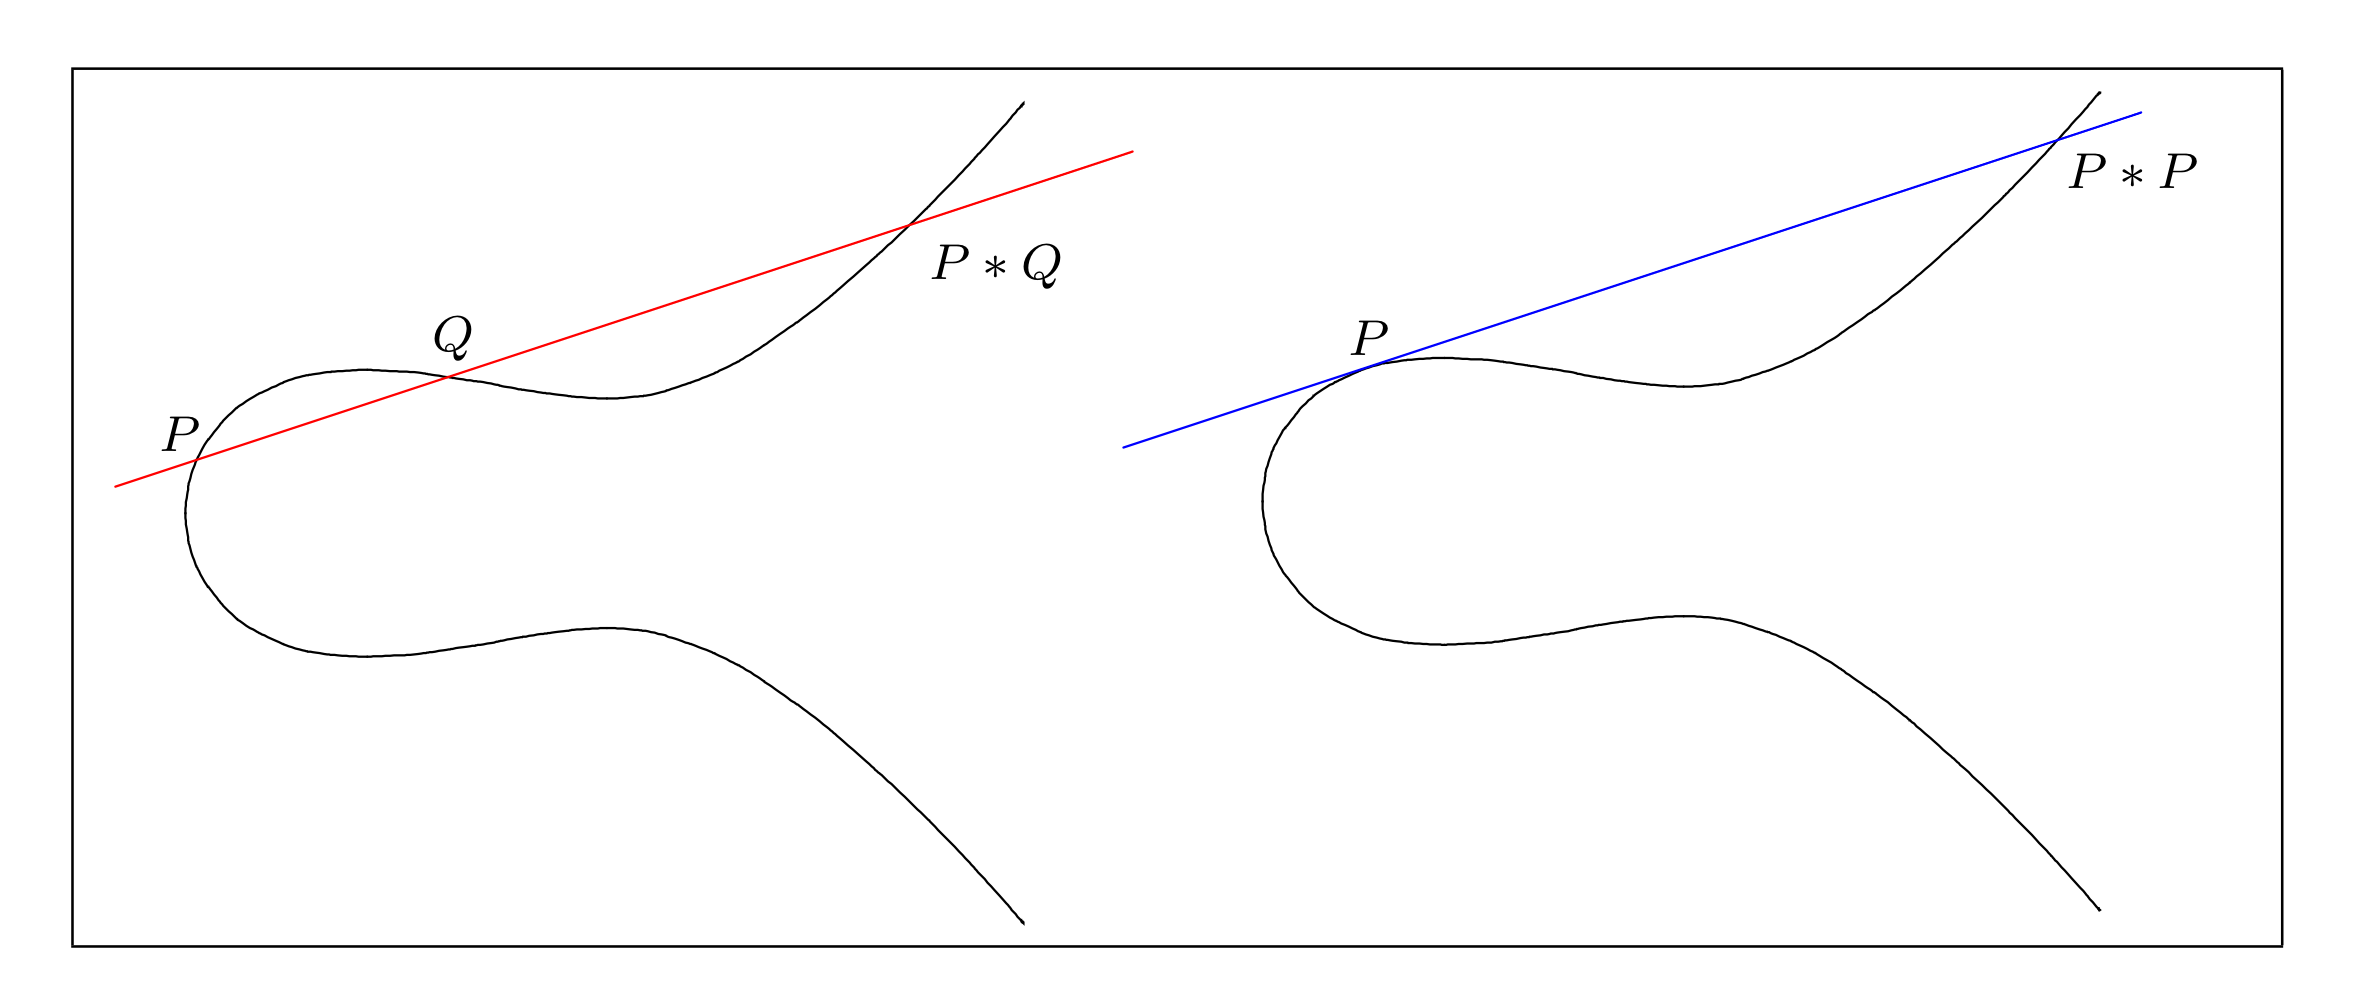
\includegraphics[width=0.8\textwidth]{cordesTangentes}
    \caption{Illustration de la loi des cordes-tangentes}
    \label{fig:cordesTangentes}
\end{figure}

On peut remarquer que sur la Figure \ref{fig:cordesTangentes}, une droite verticale
àla courbe $E$ ne semble
pas la couper en un troisième point. Ceci est lié à la difficulté de représenter le plan
projectif $\mathbb{P}_{2}$ sur un plan. Ce troisième point existe, et appartient à la droite infini
$\mathbb{P}_{1}$. Pour une courbe elliptique il correspond au $\mathcal{O}$.

\begin{remarque}
    Le meilleur moyen de considérer $\mathbb{P}_{1}$ est de se représenter ses éléments comme
    l'ensemble des directions possibles des droites du plan affine. Dans le cas particulier
    des courbes elliptiques, on a vu que $P_{1}$ se limite à un seul élément, que l'on a noté
    $\mathcal{O}$, qui correspond à la direction des droites verticales.
\end{remarque}

\begin{proposition}
    \label{prop:propasso}
    
    Pour tous points $P_1,P_2,Q_1$ et $Q_2$ de $E(K)$, on a :
    \[
    f(f(P_1,P_2),f(Q_1,Q_2)) = f(f(P_1,Q_1),f(P_2,Q_2))
    .\] 

    Pour une démonstration de ce résultat, voir 
\end{proposition}

% \subsection{Point de vue algébrique}
\begin{proposition}
    \label{prop:secTanAlg}
    
    Soient $P$ et $Q$ des points de $E$. Soit $D$ la droite de $\mathbb{P}^2$ passant par $P$ et $Q$ si $P \neq Q$, ou bien la tangente à $E$ en $P$ si $P = Q$. On a
    \[
    D \cap E = \left\{ P, Q, f(P,Q) \right\}
    ,\] 
    où $f(P,Q)$ désigne le point de $E$ défini par les conditions suivantes.
    \begin{description}
        \item[1)] Supposons $P \neq Q, \ P \neq O$ et $Q \neq O$.
            \begin{description}
                \item[i)] Supposons $x_{P} \neq x_{Q}$. Posons
                    \[
                    \lambda = \frac{y_{P} - y_{Q}}{x_{P} - x_{Q}} \text{ et } \nu = \frac{x_{P}y_{Q} - x_{Q}y_{P}}{x_{P} - x_{Q}}
                    .\] 

On a 
\begin{align}
    \label{eq:interne1}
f(P,Q) = \left[ \lambda - x_{P} - x_{Q}, \lambda \left( \lambda^2 - x_{P} - x_{Q} \right) + \nu, 1 \right]
.\end{align}
                \item[ii)] Si $x_{P} = x_{Q}$, on a $f(P,Q) = O$.
            \end{description}
        \item[2)] Supposons $P \neq O$ et $Q = O$. On a
            \begin{align}
                \label{eq:interne2}
            f(P,O) = \left[ x_{P}, -y_{P}, 1 \right]
            .\end{align}
            De même, si $P = O$ et $Q \neq O$, on a $f(O,Q) = \left[ x_{Q}, -y_{Q}, 1 \right]$
        \item[3)] Si $P = Q = O$, on a $f(O,O) = O$.
        \item[4)]  Supposons $P = Q$ et $P \neq O$.
            \begin{description}
                \item[i)] Si $y_{P} = 0$, on a $f(P,P) = O$.
                \item[ii)] Supposons $y_{P} \neq 0$. Posons
                    \[
                    \lambda = \frac{3x_{P}^3 + a}{2y_{P}} \text{ et } \nu = \frac{-x_{P}^3 + ax_{P} + 2b}{2y_{P}}
                    .\] 
On a
\begin{align}
    \label{eq:interne3}
f(P,P) = \left[ \lambda^2 - 2 x_{P}, \lambda\left( \lambda^2 - 2x_{P} \right) + \nu, 1 \right]
.\end{align}
            \end{description}
    \end{description}
\end{proposition}

\begin{demonstration}
    \begin{description}
        Soient $P = \left[ x_{P}, y_{P}, 1 \right]$ et $Q = \left[ x_{Q}, y_{Q}, 1 \right]$ des points de $E$ tels qu'ils sont distincts. Alors il existe une droite $D \in \mathbb{P} ^2$ qui passe par $P$ et $Q$.
        \item[1)] Supposons $P \neq Q$, $P \neq O$ et $Q \neq O$. Donc comme $D$ existe, il
            existe un point $M \in D \cap E$ et on cherche donc à trouver ses coordonnées.
            \begin{description}
        \item[i)] Supposons $x_{P} \neq x_{Q}$. 
            Comme $P,Q \neq O$, le point à l'infini n'appartient pas à $D$. Comme $M \in D$, il est de la même forme que $P$ et $Q$.
            Posons $M = \left[ x_0, y_0, 1 \right]$ avec $x_0$, $y_0$ des coordonnées sur $\overline{K}$.

            Comme $M \in E$, on a la première égalité
            \begin{align}
                \label{eq:droite} 
             y_0^2 = x_0^3 + ax_0 + b 
            .\end{align}
            Ensuite avec $M \in D$ d'après le lemme \ref{lem:lemme2}  on a la matrice suivante
            \[
                \begin{pmatrix}
                    x_P & x_Q & x_0 \\
                    y_P & y_Q & y_0  \\
                    1   & 1   & 1
                \end{pmatrix}
            ,\] 
           qui nous permet d'obtenir une seconde égalité.
           \begin{align*}
               \left( y_P - y_Q \right)x_0 - \left( x_P - x_Q \right)y_0 + \left( x_P y_Q - x_Q y_P \right) &= 0 \\
               y_0 = \frac{y_P - y_Q}{x_P - x_Q}x_0 + \frac{x_P y_Q - x_Q y_P}{x_P - x_Q}
           .\end{align*}
           Posons 
           \[
           \lambda = \frac{y_P - y_Q}{x_P - x_Q} \quad \text{et} \quad \nu = \frac{x_P y_Q - x_Q y_P}{x_P - x_Q}
           .\] 
           Donc l'équation de D est de la forme
           \[
           y = \lambda x + \nu z
           ,\] 
           c'est-à-dire dans notre cas on a
           \[
           y_0 = \lambda x_0 + \nu
           .\] 
           En remplacent dans \eqref{eq:droite}, il vient
           \begin{align*}
               \left( \lambda x_0 + \nu  \right)^2 = x_0^3 + ax_0 + b \\
               \lambda^2 x_0^2 + 2\lambda \nu x_0 + \nu^2 = x_0^3 + ax_0 + b \\
               x_0^3 - \lambda^2 x_0^2 + \left( a - 2\lambda \nu  \right)x_0 + b - \nu^2 = 0
           .\end{align*}
           Donc $x_0$ est une racine du polynôme
            \[
           H = X^3 - \lambda X^2 + \left( a - 2\lambda\nu \right)X + b - \nu^2
           .\] 
           On remarque que $H(x_P) = H(x_Q) = 0$ donc $x_p$ et $x_q$ sont aussi des racines de $H$.
           Par les relations coefficients racines obtient la valeur de $x_0$
           \begin{align*}
               x_0 + x_P + x_Q = - \left( - \lambda^2 \right) \\
               x_0 = \lambda^2 - x_P - x_Q
           .\end{align*} 
           Ainsi les racines de $H$ sont
           \[
           x_P, \quad x_Q \quad \text{et} \quad \lambda^2 - x_P - x_Q
           .\] 
           Il en résulte que $D \cap E$ est formé de $P$, et du point $M = f(P,Q)$.
           Donc  
           \begin{align*}
               f(P,Q) &= \left[ x_0, y_0, 1 \right] \\
                      &= \left[ \lambda^2 - x_P - x_Q, \lambda x_0 + \nu, 1 \right] \\
                      &= \left[ \lambda^2 - x_P - x_Q, \lambda\left( \lambda^2 - x_P - x_Q \right), 1\right]
           .\end{align*}
           D'où l'assertion.
       \item[ii)] Supposons $x_P = x_Q$. Comme $P$ et $Q$ sont distinct, on a alors $y_P = - y_Q$.
               D'après le lemme \ref{lem:lemme2} , la matrice suivante
               \[
                   \begin{pmatrix} x_P & x_Q & x \\
                   y_P & - y_Q & y \\
               1 & 1 & z
           \end{pmatrix} 
               .\] 

               D'où l'équation de la droite suivante
               \begin{align*}
                   2y_Px - 2y_Px_Pz &= 0 \\
                   x &= x_Pz
               .\end{align*}
               Donc le point $O$ est aussi un point de la droite $D$ donc de $D \cap E$.  Soit $M \in  D \cap E$ distincts de $O$. Si $M = \left[ 0,1,0 \right]$, d'après la situation on a $x_0 =
               x_P$ et $y_0 = \pm y_P$, donc $M = P$ ou $M = Q$. Or on a $P,Q \neq O$. Donc on a nécessairement $M = O$. Ainsi on a bien $D \cap E = \left\{ P, Q, f(P,Q)= O \right\}$, d'où
               l'assertion dans ce cas ci.
            \end{description}
        \item[2)] Supposons $P \neq O$ et $Q = O$. Donc d'après lemme \ref{lem:lemme2} , on a
            \[
            \begin{pmatrix}
                x_P & 0 & x \\
                y_P & 1 & y \\
                1   & 0 & z
            \end{pmatrix}
            .\] 
            À partir de la deuxième ligne on obtient l'équation de la droite suivante
            \begin{align*}
                x_Pz - x &= 0 \\
                x &= x_Pz
            .\end{align*}
            Si $M = \left[ x_0, y_0, 1 \right]$ est un point de $D \cap E$, on a donc $x_0 = x_P$ d'où $y_0 = \pm y_P$.
        On a ainsi $D \cap E = \left\{ P, O, f(P,O) \right\}$, où $f(P,O) = \left[ x_P, - y_P, 1 \right]$.
    \item[3)] Supposons $P = Q = O$, par le lemme \ref{lem:lemme4}  la tangente $D$ à E au point $O$ à pour $z = 0$. Par suite, $O$ est le seul point de $D \cap E$, d'où $f(O,O) = O$.
    \item[4)] Supposons $P = Q$ et $P \neq O$. L'équation de la tangente $D$ à $E$ en $P$ a donc pour équation 
        \[
        F_{X}(P)\left( x - x_Pz \right) + F_{Y}(P)\left( y - y_Pz \right) = 0
        .\] 
        \begin{description}
            \item[i)] Si $y_P = 0$, on a
                \[
                x_P^3 + ax_P + b = 0
                .\] 
                Donc $x_P$ est racine simple de ce polynôme. De plus, $F_{X}(P) \neq 0$.
                En effet, si $F_{X}(P) = 0$ on a
                \begin{align*}
                    - \left( 3x_P^2 + a \right) &= 0 \\
                    x_P^2 = - \frac{a}{3}
                ,\end{align*}
                ce qui est absurde.

                Ainsi à partir de l'équation de la tangente $D$ on a
                \begin{align*}
                    F_{X}(P)\left( x - x_Pz \right) = 0 &\implies \left( F_{X}(P) = 0\right) \ou \left( x - x_Pz = 0 \right) \\
                                                        &\implies x - x_Pz = 0
                .\end{align*}
                Donc pour $D$ on a 
                \[
                D : x = x_Pz
                .\] 
                Le seul point de $D \cap E$ distinct de $P$ est donc le point $O$, d'où $D \cap E = \left( P,O \right)$, d'où l'assertion.
            \item[ii)] Supposons $y_P \neq 0$. Du lemme \ref{lem:lemme4}  et de l'équation $b = y_P^2 - x_P^3 - ax_P$ on obtient
                \begin{align*}
                    - \left( 3x_P^2 + a \right) \left( x - x_Pz \right) + 2y_P\left( y - y_Pz \right) &= 0 \\
                    - 3x_P^2x + 3 x_P^3z - ax + ax_Pz + 2y_Py - 2y_P^2z &= 0 \\
                    2y_Py = 3x_P^2x - 3x_P^3z + ax - ax_Pz +2y_P^2z \\
                    2y_Py - ax_Pz = 3x_P^2x + ax - x_P^3z + 2b \\
                    y = \frac{3x_P^2 + a}{2y_P}x + \frac{- x_P^3 + ax_P + 2b}{2y_P}z
                .\end{align*}
                On pose $\lambda = \frac{3x_P^2 + a}{2y_P}$ et $\nu = \frac{- x_P^3 + ax_P + 2b}{2y_P}$ et on obtient l'équation de $D$, c'est-à-dire
                \[
                y = \lambda x + \nu z
                .\] 
                Le point $O$ n'est donc pas sur $D$. Soit $M = \left[ x_0, y_0, 1 \right]$ un point de $E \cap D$. On a par le même raisonnement que dans le cas (1-i) (utilise ref?) les deux équations suivantes
                \[
                y_0^2 = x_0^3 + ax_0 + b \quad \text{et} \quad y_0 = \lambda x_0 + \nu
                .\] 
                Par suite $x_0$ est une racine du polynôme
                \[
                G = X^3 - \lambda^2 X^2 + \left( a - 2\lambda\nu  \right)X + b - \nu^2
                .\] 
                Le polynôme dérivé de $G$ est
                \[
                G' = 3X^2 - 2\lambda^2 X + a - 2\lambda\nu
                .\] 
                On a
                \[
                    \begin{cases}
                G(x_P)=(0) \iff x_P^3-\lambda^2x_P^2+\left( a-2\lambda\nu \right)X+b-nu^2=0 \\
                y_P^2=x_P^3+ax_P+b \implies b=y_P^2-x_P^3-ax_P \quad \text{et} \quad y_P=\lambda x_P + \nu \implies \nu = y_P - \lambda x_P
                    \end{cases}
                .\] 
                Donc,
                \begin{align*}
                    G(x_P) &=x_P^3-\lambda^2x_P^2+\left( a-2\lambda\left( y_p-\lambda x_P \right)  \right) x_P + y_P^2-x_P^3-ax_P-\left( y_P -\lambda x_P \right) ^2\\
                    &= x_P^3-\lambda^2 x_P^2+ax_P-2\lambda x_Py_P+2\lambda^2x_P^2+y_P^2-x_P^3-ax_P-y_P^2+2\lambda x_Py_P -\lambda^2x_P^2 \\
                    &= 2\lambda^2x_p^2 
                .\end{align*}
                Par suite,
                \begin{align*}
                    G'(x_P)=0 &\iff 3x_P^2-G(x_P)+a-2\lambda\nu =0 \\
                              & \iff G(x_P) = 3x_P^2+a-2\lambda\nu \\
                              & \iff G(x_P)=0 \\
                              & \iff x_P \text{ racine de G}
                .\end{align*}
Ainsi, $x_P$ est une racine d'ordre au moins $2$ de $G$. Les racines de $G$ sont donc 
\[
x_P \quad \text{et} \quad \lambda^2-2x_P
.\] 
On obtient donc par le même raisonnement que (1-i) la formule annoncé.
        \end{description}
    \end{description}
\end{demonstration}

On obtient alors une loi de composition interne sur $E$, appelée loi de composition des
cordes-tangentes, $f\ :\ E\times E \to E$ qui à tout couple de point $(P,Q)$ de la courbe
associe le point d'intersection de la corde ou tangente associé $f(P,Q) \in E$ défini
dans la proposition \ref{prop:secTanGeo} 

\begin{exemple}
\end{exemple}

\section{Loi de groupe}

% \subsection{Point de vue géométrique}

\begin{theoreme}
    Soit un corps $K$. Soit $E$ une courbe elliptique définie sur $K$. Soient $P$ et $Q$ deux
    points de cette courbe. Alors, 

    \[
    P + Q = f(f(P,Q),\mathcal{O})
    ,\] 
    définit une structure de groupe commutatif ayant $\mathcal{O}$ pour élément neutre
    de la loi.
\end{theoreme}

\begin{figure}[h]
    \centering
    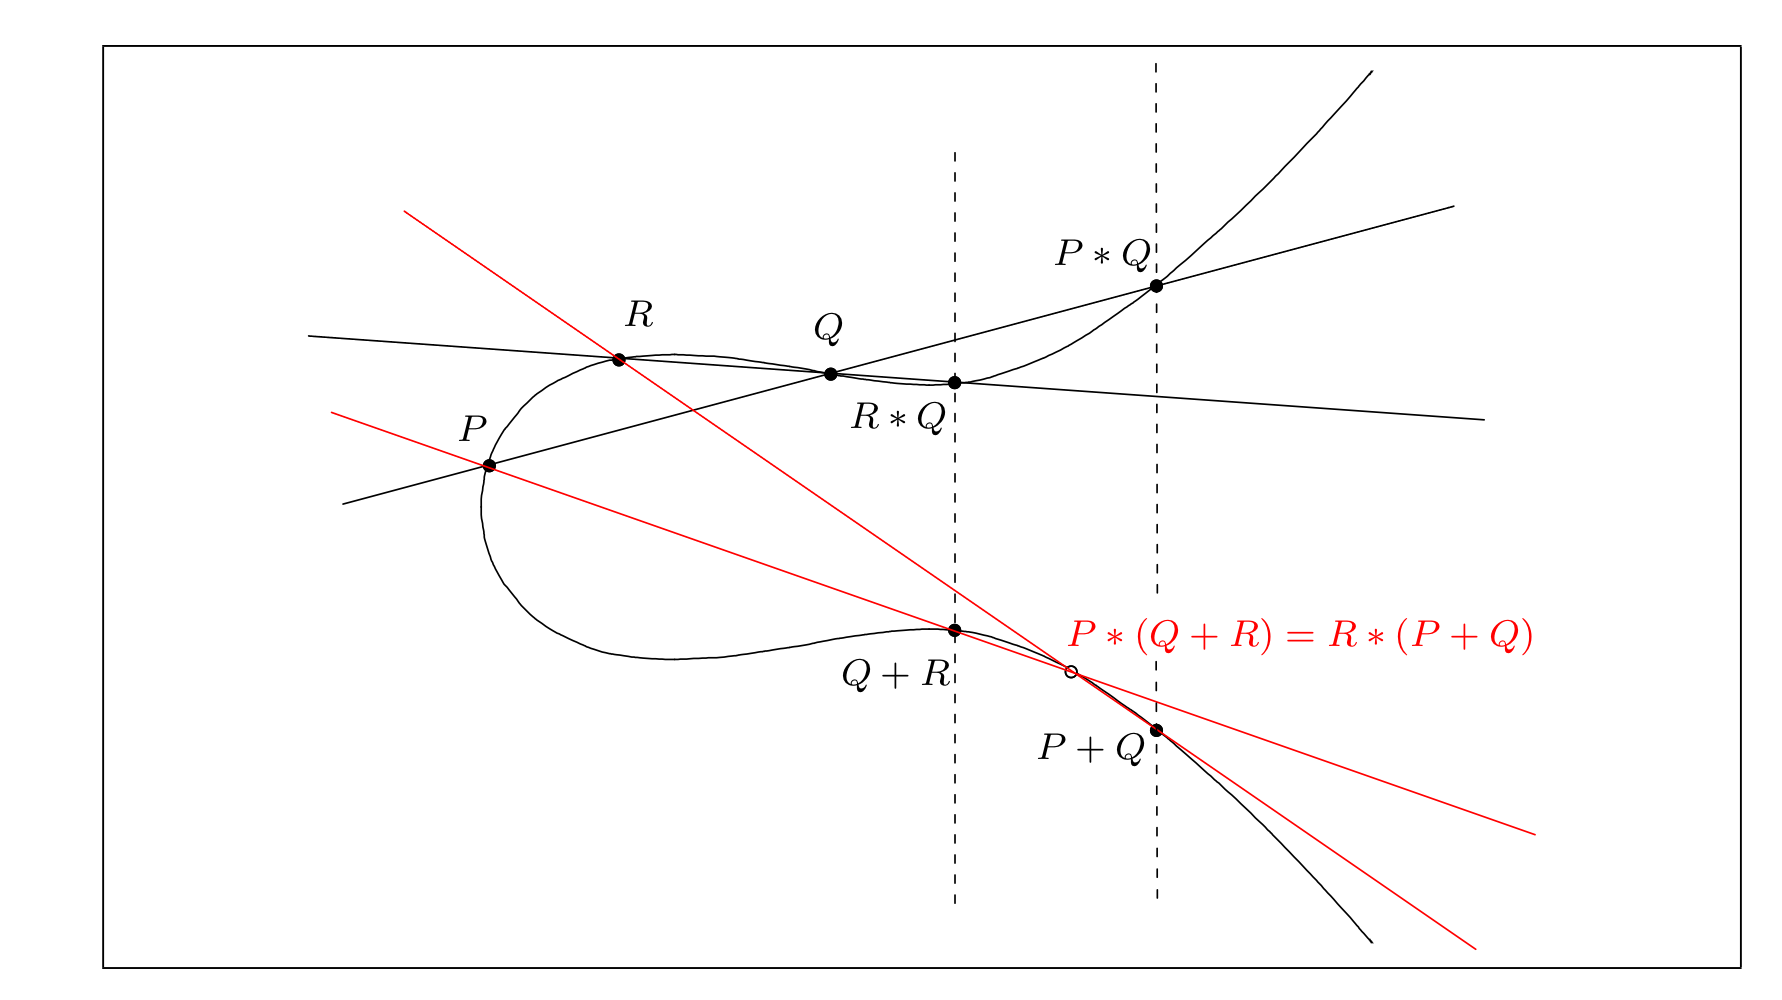
\includegraphics[width=0.8\textwidth]{associativiteGeo}
    \caption{Illustration de l'associativité de la loi de groupe}
    \label{fig:associativiteGeo}
\end{figure}

\begin{figure}[h]
    \centering
    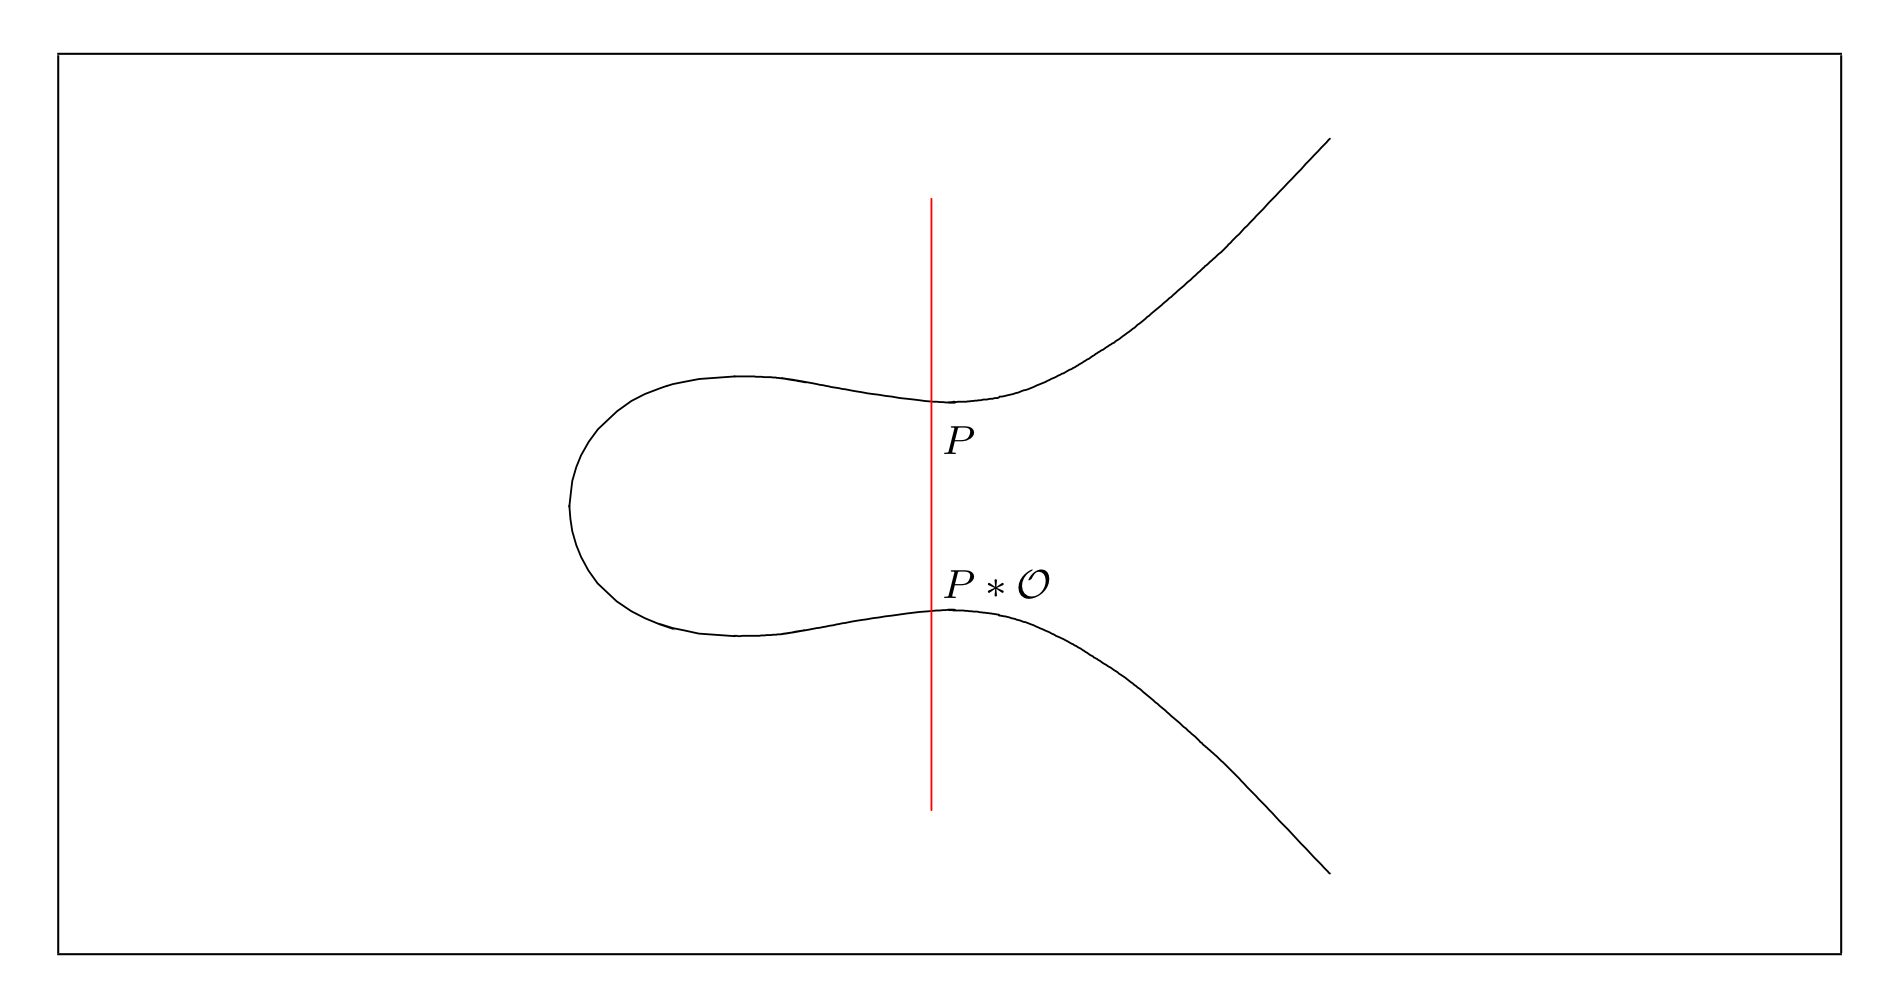
\includegraphics[width=0.6\textwidth]{P+O}
    \caption{L'élément neutre de la loi de groupe}
    \label{fig:P-O}
\end{figure}

\begin{demonstration}
    \begin{enumerate}
        \item La loi $+$ est bien interne puisque $P + Q$ est l'intersection entre la courbe et
            une droite, c'est à dire un point de la courbe.

        \item La loi $+$ est associative (voir Figure \ref{fig:associativiteGeo}). En effet, si $P,Q$ et $R$ sont trois
            point de la courbe, on a

            \begin{align*}
            f(P,f(Q+R)) &= f(P,f(f(Q,R),\mathcal{O})) \\
            &= f(f(f(P,Q),Q),f(f(Q,R),\mathcal{O})) \text{ car } P = f(f(P,Q),Q) \\
            &= f(f(f(P,Q),\mathcal{O}),f(f(Q,R),Q)) \text{ voir la proposition
            \ref{prop:propasso} } \\
            &= f(f(f(P,Q),\mathcal{O}),R) \text{ voir la Figure \ref{fig:associativiteGeo}} \\
            &= f(f(P+Q),R)
            .\end{align*}

            En appliquant $\mathcal{O}$ sur les deux membres de l'égalité, on trouve

            \[
            P + (Q+R) = (P+Q) + R
            .\] 

        \item L'élément $\mathcal{O}$ est l'élément neutre de la loi additive (voir Figure
            \ref{fig:P-O}). 

            En effet,

            \[
            P + \mathcal{O} = f(f(P,O)O) = P \quad \text{et} \quad \mathcal{O}+P =
            f(f(\mathcal{O},P),\mathcal{O}) = P
            .\] 

        \item Tout point $P$ possède un inverse pour la loi $+$. En effet, il faut vérifier que
            le point $-P= f(f(\mathcal{O},\mathcal{O}),P)$ est bien l'inverse de $P$ 

            \begin{align*}
                P + (-P) &= f(f(P,-P),\mathcal{O}) \\
                &= f(f(f(P,f(f(\mathcal{O},\mathcal{O}),P),\mathcal{O}))) =
                f(f(\mathcal{O},\mathcal{O}),\mathcal{O}) =
                \mathcal{O}+\mathcal{O}=\mathcal{O}  \\
                (-P) + P &= f(f(-P,P),\mathcal{O}) \\
                &= f(f(f(f(\mathcal{O},\mathcal{O}),P),P),\mathcal{O}) =
                f(\mathcal{O},f(\mathcal{O},\mathcal{O})) + \mathcal{O}+\mathcal{O}=
                \mathcal{O} \\
            .\end{align*}

        \item Enfin la loi $+$ est commutative. C'est à dire que si $P$ et $Q$ sont deux
            points de la courbe, on a

            \[
            P + Q = f(f(P,Q),\mathcal{O}) = f(f(Q,P),\mathcal{O}) = Q + P
            .\] 
    \end{enumerate}    
\end{demonstration}

Les propiétés de la loi de groupe sur une courbe elliptique sont représentées sur la Figure
\ref{fig:loiGroupe}.

\begin{figure}[H]
    \centering
    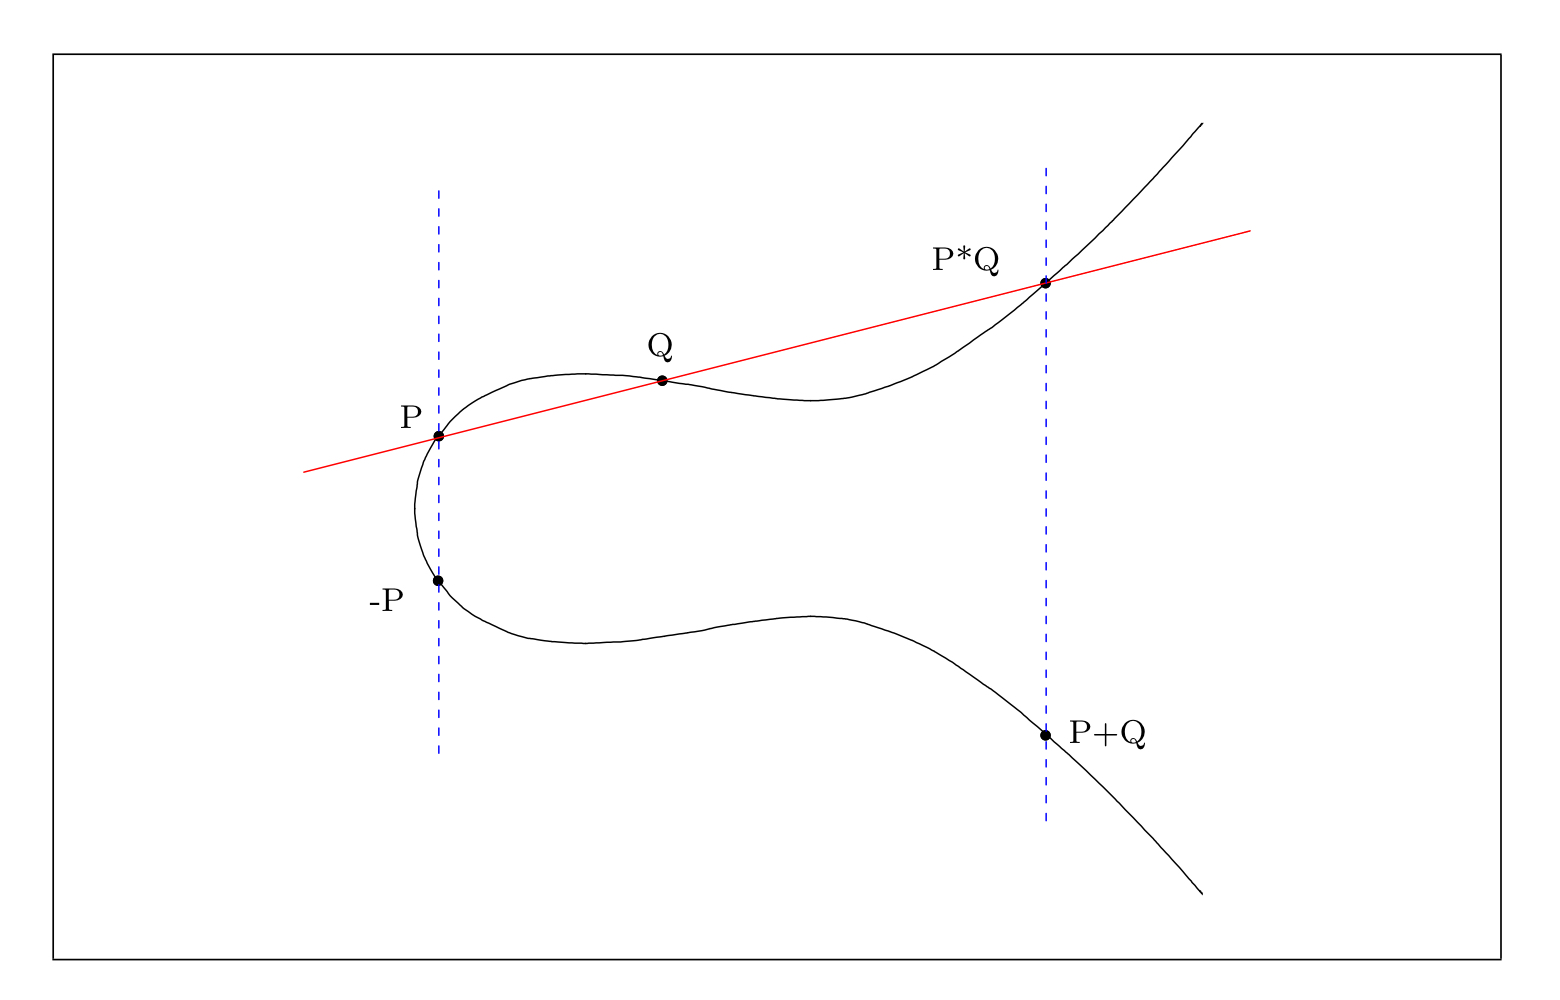
\includegraphics[width=0.8\textwidth]{loiGroupe}
    \caption{La loi de groupe + sur l'ensemble des points rationnels d'une courbe
    elliptique}
    \label{fig:loiGroupe}
\end{figure}

Considérons comme précédemment $a$ et $b$ des éléments de $K$ tels que $4a^3+27b^2\neq 0$ et $E$ la courbe elliptique définie sur $K$ d'équation
\[
y^2=x^3+ax+b
.\] 
Notons $+$ la loi de composition interne sur $E$, définie pour tous $P$ et $Q$ dans $E$ par l'égalité
\begin{align}
    \label{eq:groupe}
    P+Q=f(f(P,Q),O)
.\end{align}

\begin{theoreme}
    \label{th:theoreme1}
    Le couple $\left( E,+ \right) $ est un groupe abélien, d'élément neutre $O$. La loi interne $+$ est décrite explicitement par les formules suivantes.

    Soient $P$ et $Q$ des points de $E$ distincts de $O$. Posons $P=\left( x_P,y_P \right) $ et $Q=\left( x_Q,y_Q \right) $.

    \begin{description}
        \item[1)] Supposons $x_P\neqx_Q$. Posons 
            \[
            \lambda=\frac{y_P-y_Q}{x_P-x_Q} \quad \text{et} \quad \nu=\frac{x_Py_Q=x_Qy_P}{x_P-x_Q}
            .\] 
            On a 
            \begin{align}
                \label{eq:add1}
            P+Q=\left( \lambda^2-x_P-x_Q,-\lambda\left( \lambda^2-x_P-x_Q \right) -\nu  \right) 
            .\end{align}
            \item[2)] Si $x_P=x_Q$ et $P\neqQ$, on a $P+Q=O$.
            \item[3)] Supposons $P=Q$ et $y_P\neq 0$. Posons 
                \[
                \lambda=\frac{3x_P^2+a}{2y_P} \quad \text{et} \quad \nu=\frac{-x_P^3+ax_P+b}{2y_P}
                .\] 
                On a 
                \begin{align}
                    \label{eq:add2}
                2P=\left( \lambda^2-2x_P,\lambda\left( -\lambda^2-2x_P \right) -\nu \right) 
                .\end{align}
        \item[4)] Si $P=Q$ et $y_P=0$, on a $2P=O$.
        \item[5)] L'opposé de $P$ est le point
            \begin{align}
                \label{eq:add3}
                -P=\left( x_P,-y_P \right) 
            .\end{align}
    \end{description}
\end{theoreme}

\begin{demonstration}
    \begin{description}
        \item[1)] Supposons $x_P\neqx_Q$, compte tenu de \eqref{eq:groupe}, \eqref{eq:interne1} et \eqref{eq:interne2} on a
            \[
            \begin{cases}
                \eqref{eq:interne1} \iff f(\left[ \lambda^2-x_P-x_Q,\lambda\left( \lambda^2-x_P-x_Q \right) +\nu,1 \right] , \left[ 0,1,0 \right] ) \\
                \eqref{eq:interne2} \iff f(P,O)=\left[ x_P,-y_P,1 \right] 
            \end{cases}
            .\] 
            On retrouve bien la formule \eqref{eq:add1}.
        \item[2)] Supposons $x_P=x_Q$ et $P\neq Q$ c'est à dire $y_P\neq y_Q$.

            D'après la proposition \ref{prop:secTanGeo}  (1-i), on a $f(P,Q)=O$ donc $f(f(P,Q),O)=f(O,O)=O$. D'où la formule énoncé.
        \item[3)] Supposons $P=Q$ et $y_P\neq 0$, en prenant compte \eqref{eq:groupe} , \eqref{eq:interne2} et \eqref{eq:interne3} on obtient
            \[
            \begin{cases}
                \eqref{eq:interne3} \iff f(\left[ \lambda^2-2_x_P,\lambda\left( \lambda^2-2x_P \right) +\nu,1 \right] ,\left[ 0,1,0 \right] )\\
                \eqref{eq:interne2} \iff f(P,O)=\left[ x_P,-y_P,1 \right] 
            \end{cases}
            .\] 
            Ce qui permet de retrouver la formule \eqref{eq:add2}. 
        \item[4)] Supposons $P=Q$ et $y_P=0$, d'après l'assertion (4-i) de la proposition \ref{prop:secTanGeo} , on a $f(P,P)=O$ d'où $2P=f(f(P,P),O)=f(O,O)=O$. 
        \item[5)] Pour l'opposer on cherche un point $M \in E$ tel que $P\neq M$ et $P,Q\neq O$ d'après le théorème énoncé assertion 2) on a donc $x_P = x_M$ et donc nécessairement $y_M=-y_P$ donc le point recherché est $M=\left( x_M,y_M \right) = \left( x_P,-y_P \right) =-P$. 
    \end{description}
\end{demonstration}

\begin{exemple}
    mettre exemple de calcul de $2P$ pour la suite
\end{exemple} 

